\documentclass[12pt]{article}

\usepackage[utf8]{inputenc}
\usepackage[bulgarian]{babel}
\usepackage{graphicx}
\usepackage{sidecap}  %required for side captions
\usepackage{amssymb}
\usepackage{amsmath}
\usepackage{hyperref}
\usepackage{commath}  
\usepackage[top=1.3in, bottom=1.5in, left=1.3in, right=1.3in]{geometry}


\begin{document}
	\begin{center}
        \LARGE{\textbf{Тема: Разширяване на проекта по Web технологии за - Project Estimation}}
        
        \bigskip
        \Large{Предмет: Приложно-програмни интерфейси за работа с облачни архитектури с Амазон Уеб Услуги (AWS)}
        
        \medskip
        \Large{Изготвил: Диана Иванова, фн: 81426, имейл: didi.e.ivanova@gmail.com}
        
        \medskip
        \Large{Лектор: Милен Петров, година: 2020}
        
        \bigskip
	\end{center}
    
    
   \newpage
    \tableofcontents
    \bigskip
    \bigskip
    \newpage
  
\section{Условие} 

\noindent Документиране на разгръщане на съществуващ проект по уеб технологии (Project Estimation) - под формата на AWS услуги, разширяване на на проекта с поне една услуга на амазон и интегриране с някоя от другите услуги на AWS.

\medskip

\section{Въведение}

 В настоящата документация е представено описание на системата и
разгръщането и върху облачна архитектура, инсталация и ръководство. 
 Project estimation е система за възлагане и автоматично оценяване 
 на задачи и проекти, както и за визуално представяне на данните 
 под формата на burn-down chart. Използваните услуги и тяхното 
 приложение са както следва:  
 

\begin{itemize}
    \item Потребителите могат да се 
 регистрират и да влизат в уеб-сайтът с име и парола, като
 за целта е използвана aws услугата Cognito.
    
    \item  Базите от данни 
 ще бъдат разположени в облака и ще се оперира с тях посредством
 Amazon RDS..
    
    \item Останалата част от програмата работи сървърфул
 върху инстанция на EC2.
\end{itemize}

\section{Теория}

\textbf{Разгръщане:}\medskip

Използвайки Amazon RDS за MySQL, базата данни ще бъде върху отделна инстанция от тази на уеб сървъра, така че те няма да се състезават за ресурси. Amazon RDS за MySQL има автоматизирани резервни копия и ъпдeйти, спомагащи за администрацията на базите данни.
Security group-ата на RDS има Inbound правило за достъп от тип MySQL на порт 3306 с източник security group-ата на EC2 инстанцията. По този начин EC2 достъпва данните и може да прави заявки към RDS базата данни. От своя страна security групата на EC2 има за правило Inbound правило тип HTTP, порт 80 и източник всеки, като позволява да може да се достъпва уеб-сайтът от всички. EC2 има и SSH правило на порт 22 с източник моят ip адрес, за да мога да правя промени по сайтът и да го поддържам.\medskip

Аутентикацията става с помощта на AWS Cognito, като при всяка регистрация системата изпраща имейл за потвърждение към пощата на потребителя. Amazon Cognito е услуга за синхронизация на идентичността на потребителя, която позволува управление на потребителите и администрация. 
Всички скриптове, html и css документи са на EC2 инстанция, върху който работи apache сървър.\medskip

 \textbf{Функционалност:}\medskip
 
Системата за оценяване борави с два типа оценки - експертна и реална. Експертната оценка за една задача се формира на база тагове - css, event, insert into db, query from db и още. На всеки един таг съответстват часове работа (пр. event - 1, query from db - 2). Потребителят на системата въвежда реалната оценка след като завърши задача. Двата типа оценка за самия проект се формира като сума от съответните типове оценки на всички задачи по проекта. На базата на тези данни се изготвя burn down диаграма.


\section{Използвани технологии}
\begin{itemize}
   
    \item \textbf{MySQL}    - Ver 15.1 Distrib 5.5.64-MariaDB, for Linux (x86\textunderscore 64) using readline 5.1
       
     \item \textbf{PHP} - версия 7.2
     
     \item \textbf{Apache} - Apache httpd 2.4.41
     
     \item \textbf{Javascript JQuery} - version-3.1.0
     
     \item \textbf{mazon-cognito-identity-js} - version 1.31.0
   
     \item \textbf{CSS}
   
    \item \textbf{AWS EC2} -  Amazon Linux 2 AMI (HVM)
    
    \item \textbf{AWS RDS} 
    
    \item \textbf{HTML} 
    
    \item \textbf{AWS Cognito} 
     

\end{itemize}

%\newpage

\section{Инсталация и настройки}
\noindent\textbf{Стъпка 1.} Създаване на User pool в Когнито с име Еstimateme. Нека да е с атрибут имейл и верификация на имейла чрел линк. Създадете App Client с име EstimatemeApp като махнете отметката на Generate client secret опцията. Конфигурирайте 
config.js файла. Поставят се съответния регион, poolId и userPoolId. 

\medskip

\noindent\textbf{Стъпка 2.} Създаване на EC2 инстанция със следните параметри:
\begin{itemize}
\item  За AMI изберете Amazon Linux 2 AMI (HVM)
\item тип на инстанцията t2.micro
\item Създайте нова Security Group-а с име estimateme като добавите
следните правила
 1)SSH трафик от текущия Ви IP адрес за да използвате SSH протокол, за да влезнете във вашата EC2 инстанция и да конфигурате уеб страницата;
 2)HTTP трафик от всички IP адреси така че потребителите да могат да виждат Project Estimation сайтът.
\item Накрая запазете Key Pair ключа, за да можете да се логнете в EC2 инстанцията
\end{itemize}

\medskip

\noindent\textbf{Стъпка 3.} Създавайте RDS база данни. 
Изберете  \textbf{MySQL} за система за управление на бази данни (СУБД).
Изберете за шаблон (template) free tier. В Settings секцията, 
въведете \textbf{projectEstimation} за идентификатор на инстанцията
база данни. След това посочете master потребителско име и парола за Вашата база данни. 
\begin{itemize}
\item За VPC изберете „по подразбиране“
 \item За „Subnet group“ изберете \textbf{„rdsfmi“}
\item На „Публична достъпност“ изберете „Да“
\item За availability zone изберете \textbf{„eu-central-1a“}
\item За „VPC security groups” изберете “Choose existing VPC security groups” и изберете група \textbf{„sgFMI“}
\item За „Име на базата данни“ въведете \textbf{„estimateme“}
\item За криптиране изберете \textbf{„Disable encryption“}
\item На  “Enhanced monitoring” премахнете 
отметката квадратчето пред Enable Enhanced monitoring
\item За „Защита при изтриване“ премахнете отметката от квадратчето пред “Enable deletion protection”
\item Натиснете бутона Create Database
\item  Разрешете на вашия екземпляр EC2 достъп до вашата RDS база данни по следния начин: кликнете на
Security Group-ата. В inbound-таба добавете 
правило  с Type property  MYSQL/Aurora и сменете текущата стойност на security групата със \textbf{"estimateme"} security групата, която използвахте за EC2 инстанцията и запазете промените
\end{itemize}
за прикачване на sql скриптовете
от папката sqlscripts.

\noindent\textbf{Стъпка 4.} Направете SSH връзка към инстанцията.
 Въведете командата:
\medskip

\textbf{sudo yum install -y mysql}\medskip


\noindent След това намерете името на хоста за вашата RDS база данни в конзолата AWS. В детайлите на вашата RDS база данни името на хоста ще бъде показано като Endpoint в секцията Security and Connection.

\medskip Въведете командата:

\medskip
\textbf{export MYSQL\textunderscore HOST=<your-endpoint>}

\medskip

\noindent където <your-endpoint> e името на хоста

\medskip Въведете командата: 

\noindent\textbf{mysql --user=<user> --password=<password> estimateme}

\noindent заменете <user> и <password> със мастър потребителското име и паролата, които конфигурирахте при създаването на RDS базата от данни 

\begin{figure}[h!]
\centering
  \includegraphics[width=0.8\textwidth]{accessToDatabase.png}
  \caption{Access to Database using Cli}
\end{figure}


И накрая, създайте потребител на база данни за вашето
project estimation приложение и му дайте разрешение за достъп до базата данни „estimateme“.
Изпълнете следните команди във вашия терминал:

\medskip
CREATE USER 'estimateme' IDENTIFIED BY ‘password';\\
GRANT ALL PRIVILEGES ON estimateme.* TO estimateme;\\
FLUSH PRIVILEGES;\\
Exit;\\
където изберете подходяща парола за  password

\noindent\textbf{Стъпка 5.}
За да инсталирате Apache на вашата EC2 инстанция, изпълнете следната команда във вашия терминал:

\medskip
\textbf{sudo yum install -y httpd}

\medskip
\noindent За да стартирате уеб сървъра Apache, изпълнете следната команда във вашия терминал:

\medskip
\textbf{sudo service httpd start}

\medskip
\noindent Инстарирайте php: Първо проверете дали имате amazon-linux-extras. 

\medskip
\textbf{which amazon-linux-extras}

\medskip
\noindent ако ги нямате, ги инсталирайте първо

\medskip
\textbf{sudo yum install -y amazon-linux-extras}

\medskip
\textbf{sudo amazon-linux-extras enable php7.2}

\medskip
\textbf{\# yum clean metadata \&\&
sudo yum install php70u php70u-pdo php70u-mysqlnd php70u-opcache php70u-xml php70u-gd php70u-devel php70u-mysql}

\medskip
\textbf{sudo service httpd restart}

\medskip
\noindent Качете estimateme.zip на ec2 инстанцията:

\medskip
\textbf{scp -i path/to/key path/to/file user@ec2-xx-xx-xxx-xxx.compute-1.amazonaws.com:}$\sim$/. 

 \noindent след което въведете следните команди
 
 \medskip
\textbf{unzip estimateme.zip}

\medskip
\textbf{sudo cp -r main/* /var/www/html/}

\medskip
\textbf{mysql --user=<user> --password=<password> estimateme < all{\textunderscore} tables.sql}

Редактирайте конфигурациите за базата данни във файла \textbf{dbConnect.php} като попълните празните полета със съответните стойности:

\medskip
\$host = ' '; 

\medskip
\$dbname = ' '; 

\medskip
\$username = ' ';

\medskip
\$password = ' '; 

\section{Кратко ръководство за потребителя}

\begin{SCfigure}
  \centering
  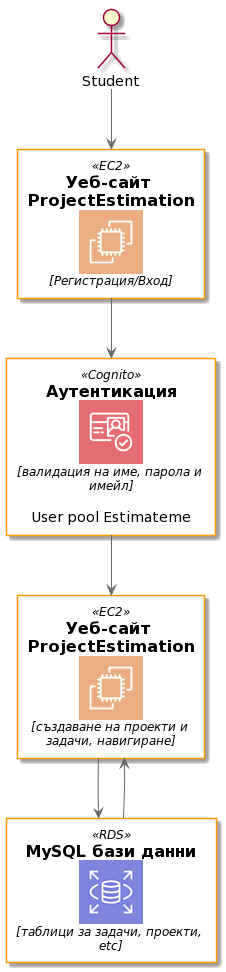
\includegraphics[width=0.35\textwidth]{81426_fig1.png}
    \caption{Диаграма - кратко ръководство на потребителя [PlantUML]}
\end{SCfigure}


Потребителят достъпва сайта на адрес:
  
  \medskip http://ec2-18-233-153-235.compute-1.amazonaws.com/register.php


Регистрация. Потребителят се регистрира със своя имейл като избира подходящо потребителско име, парола и тип-акаунт. Има два типа акаунти - за разработчици и мениджъри. Потребителят трябва да верифицира акаунта, като кликне на линка изпратен в пощата \medskipму.

Влизане в \medskipсистемата.

Потребителят може да провери текущите проекти, в които участва в страницата “Проекти”.
Ако е мениджър ще види и проектите които е създал. Само мениджърите могат да създават \medskipпроекти.

Потребителят може да разгледа детайлно всеки от проектите, в които участва като кликне върху ‘кутийката’’ със съответния проект. Страницата с описание на проекта изброява задачите в него под формата на таблица. Там потребителят може да избере статус на задачата, която му е разпределена. Т.е ако започва задачата трябва да смени статуса и на ‘in progress’ посредством падащото меню. Под таблицата (ако в нея има поне една задача) автоматично се генерира burn down chart на базата на часовете нужни за задачите и целия проект. 
\medskip


\begin{figure}[h!]
\centering
  \includegraphics[width=1\textwidth]{tasks.png}
  \caption{View project tasks}
\end{figure}


Могат да се добавят нови задачи към всеки един от проектите. 
Избира се име на задачата, възлага и се изпълнител и се добавят тагове, всеки от които носи часове трудност. Системата автоматично смята трудността на задачата според таговете, така че потребителят трябва да въведе възможно най-точните тагове за конкретната задача. Ако потребителят не е доволен от предоставената оценка, може да я смени в съответното поле. Към задачата може да се добави и описание.

\begin{figure}[h!]
\centering
  \includegraphics[width=1\textwidth]{create_task.png}
  \caption{Create new project}
\end{figure}

\medskip

В страницата “Импорт” могат да се добавят данни (за проекти и потребители) в json формат за лесно вмъкване на данни в базата. В страницата “Експорт” могат да се извличат данни за задачи по даден проект в json формат.

\begin{figure}[h!]
\centering
  \includegraphics[width=1\textwidth]{import.png}
  \caption{Import files}
\end{figure}

\medskip

Излизане от системата (Логаут).
\newpage
\section{Примерни данни}

Примерни данни за импорт на потребители и проекти със задачи към тях се съдържат във файлове demo\textunderscore file\textunderscore projects.json , demo\textunderscore file\textunderscore  users.json. 

Примерни данни за импорт на проект:

\medskip
[

   \medskip
  \{
  
  \medskip
    "name": "DEMO",
    
      \medskip
    "tasks": [
    
      \medskip
      \{
         "title": "Прикачане на изображение",
         
           \medskip
         "tags": "picture,column",
        
          \medskip
         "description": "При отваряне на модал за създаване на стая, да има кламерче за прикачане с действаща функционалност. "
         
           \medskip
      \},
        
          \medskip
      \{
      
        \medskip
         "title": "Download hyperlink",
         
           \medskip
         "tags": "hyperlink,php",
         
           \medskip
         "description": "Когато потребителят кликне на линка, да се сваля файл с име temp.png"
      \}
   ]
   
     \medskip
  \}
]


Примерни данни за импорт на потребители:

  \medskip

[
  \{
      "username": "Georgi Petrov",
      
        \medskip
      "password": "9999",
      
        \medskip
      "email": "mail\textunderscore 1@fake.com",
      
        \medskip
      "account\textunderscore type": "Manager"
    \},
    
      \medskip
    \{
        "username": "Maria Dimitrova",
        
          \medskip
        "password": "8888",
        
          \medskip
        "email": "mail\textunderscore 2@fake.com",
        
          \medskip
        "account\textunderscore type": "Developer"
    \} ]

 
\section{Описание на програмния код}

Във config.js се съдържат конфигурационните настройки за връзката с congito user  pool-ът

\medskip
\noindent window.\textunderscore config = \{ \\
    cognito: \{  \\
        userPoolId:  'example-user-pool-id', \\
        userPoolClientId: 'example-user-pool-client-id',\\ 
        region: 'example-region' \\
   \}\\ ;

\medskip
cognito-auth.js съдъра функции за event-handling при регистрация и логин. Функцията register(email, username, password, onSuccess, onFailure) добавя потребителят в user pool-а, а signin(username, password, onSuccess, onFailure)  проверява за потребителя в user-pool-a
 
  
 В dbConnect се съдържат конфигурационните данни за базата данни, както и се осъществява връзка с базата.
 
 \medskip
 \$host = '<endpoint-name>'; 

 \medskip
\$dbname = '<database-name>';

 \medskip
\$username = '<username>';

 \medskip
\$password = '<password>'; 

\begin{table}
\caption{Описание на кода по файлове}
\center
\begin{tabular} {|l|p{0.6\linewidth}| }
 \hline
 autofill.js & съдържа скрипт за автоматично попълване на полето за тагове\\\hline
change\textunderscore status.php & промяна на статуса на задачата в базата данни \\ \hline 
 createProjectScript.js & скрипт за създаване на проект - обработва събитието кликване върху бутона “създай проект”  \\ \hline
 current-project.js & обработва бутоните в текущия проект за изтриване на проекта и създаване на задачи, както и таговете\\\hline
  current\textunderscore project.php & съдържа формите за въвеждане на данни за съответния проект и неговите задачи \\\hline
  dbConnect.php & установява връзка с базата от данни\\
 \hline
 demo\textunderscore file\textunderscore projects.json & json файл с примерни данни за проекти \\
 \hline
  demo\textunderscore file\textunderscore users.json & json файл с примерни данни за потребителите\\
 \hline
 estimate\textunderscore task.php & оценява задачата на база оценките на таговете\\
   \hline
  export.php & експортиране на данните от базата във json формат \\
   \hline
  get\textunderscore all\textunderscore projects.php & форма за експортиране на файлове \\
   \hline
  graphic.php & създава графична визуализация на оценката на задачите в проект чрез burn down chart \\
   \hline
  import\textunderscore projects.php & обработка на json данните за проектите и внасянето им в базата\\ 
  \hline
  import\textunderscore users.php & обработка на json данните за потребителите и внасянето им в базата\\
  \hline
  landing\textunderscore page.php & начална страница\\
  \hline
  login.php & логин форма за попълване и  верифициране на паролата и името на текущия потребител \\ 
  \hline
  logout.php & прекъсване на текущата сесия \\
    \hline
  main.css & css на логин-а\\
    \hline
  nav\textunderscore menu.php & навигационно меню\\
    \hline
  project\textunderscore creation.php & вкарване на данните за проекта в базата данни  \\
     \hline
  project\textunderscore delete.php & изтрива проекта и прилежащите му задачи от базите от данни \\ 
     \hline
  projectsPage.php & страница със всички проекти изброени с прилежащата към тях информация\\  
     \hline
  register.php & форма за регистрация\\
     \hline
  register\textunderscore script.php & хеширане на паролите, проверява дали съществува вече такъв потребител  \\
     \hline
  tags.css & стилизира таговете \\
     \hline
  tags.js & обработва въвеждането на тагове \\
     \hline
  task\textunderscore eation.php & добавяне на задача в базите от данни \\
     \hline
  upload.php & форма за импортиране на файлове \\
     \hline
  all\textunderscore tables.sql & таблици за потребители, проекти и т.н \\
 \hline
\end{tabular}
%\label{table:ta}
\end{table}
%\caption{\label{tab:table-name}Your caption.}

\medskip


\section{Приноси на студента, ограничения и възможности за бъдещо развитие}
\begin{itemize}
   \item Възможност за бъдещо развитие е да се добавят още функционалности чрез Cognito, като промяна на парола, управление на акаунт и т.н. Също може да се създаде Auto Scaling група, която да позволява scale out, в случай, че потребителите станат твърде много за един сървър.
  \item Миграцията от EC2 на Lambda Serverless би била трудна, тъй като Lambda не работи с PHP, а основният сървърен език използван за проекта е PHP. 
   \item Приноси на студента: 
Разгръщане върху EC2; свързване с RDS база данни; осигуряване на достъп то сайтът чрез Cognito User pool; валидация на регистрация и логин
Визуализация на оценката  чрез burndown chart - оставащи усилия(часове) - спрямо оставащи дни; 
навигационно меню;
част от таблиците в базите от данни;
създаване на проект;
визуализация на проекти в ‘кутийки’;
изготвяне на документация;
тестване;


\end{itemize}
\medskip

\section{Какво научих}
Научих се как да работя с AWS Congito и User pools, както и да ползвам библиотеките за услагата предоставени от AWS (aws-amplify). Вече мога и да правя MySQL заявки през CLI, да създавам инстанции на бази данни в AWS RDS. Научих се да качвам файловете от локалната машина към ЕC2, както и да настройвам Security Group-и така, че инстанциите да получават подходящ достъп. Мога да свързвам EC2 със RDS и по този начин да отделя базата от изчислителната машина. 


\newpage 

\section{Списък с фигури и таблици}

\listoftables

\listoffigures

\section{Използвани източници}

\noindent\href{https://github.com/aws-amplify/amplify-js/tree/master/packages/amazon-cognito-identity-js}{[1] Amazon Cognito Identity SDK for JavaScript}
\\\href{https://github.com/awslabs/aws-icons-for-plantuml}{[2] Икони за plantuml}
\\\noindent\href{https://aws.amazon.com/premiumsupport/knowledge-center/ec2-install-extras-library-software/}{[3] Инстаналация на PHP 7.2}
\\\noindent\href{https://docs.aws.amazon.com/cognito/latest/developerguide/what-is-amazon-cognito.html} {[4] AWS Cognito, create and manage user pools}
\\\noindent\href{https://docs.aws.amazon.com/AmazonRDS/latest/UserGuide/CHAP_GettingStarted.CreatingConnecting.MySQL.html}
{[5] AWS RDS, създаване, управление на бази от данни}
\\\noindent\href{https://learn.fmi.uni-sofia.bg/pluginfile.php/247022/mod_resource/content/0/Exercise\%2012\%20-\%20RDS\%20-\%20Exercise.pdSf }
{[6] AWS RDS, упражнение 10 в курса}
\\\noindent\href{https://docs.aws.amazon.com/AmazonRDS/latest/UserGuide/USER_VPC.Scenarios.html}{[7]Достъпване на RDS база данни от EC2 инстанция}

 
\medskip



\bigskip


\end{document}